% !TEX TS-program = lualatex
% !TEX encoding = UTF-8 Unicode

\documentclass[]{einformatica}
\usepackage{graphicx}
\usepackage{soul}
\usepackage{booktabs}
\usepackage{hyphenat}
\usepackage[all]{nowidow}
\usepackage{tabularx}
\usepackage{floatrow}
\floatsetup[table]{style=plain,capposition=top}
\renewcommand\topfraction{.95}
\renewcommand{\textfraction}{0.05}
\usepackage{refcount} 
\usepackage[noadjust]{cite}

\usepackage{xcolor}
\usepackage{cleveref}
\usepackage{amsmath}
\usepackage{amssymb}

% Please, add only really required packages here

\begin{document}

\title{Text-to-SQL Dataset Quality Assessment: The First Open-Source Validation Framework}

\shortauthorshead{Sabadosh et al.}

\eIsubmitted{1 Nov. 2024} 
\eIrevised{15 Jan. 2025} 
\eIaccepted{20 Feb. 2025}
\eIpublished{1 Mar. 2025} 
\eIyear{2025}

\EIauthorI
   {Volodymyr}
   {Sabadosh}
   {Your Institution, Your Country}
   {vsababadosh@gmail.com}
   {0009-0006-9933-444X}
   {*} %  if star present means corresponding author

\EIauthorII
   {Vladyslav}
   {Kotsovsky}
   {Uzhhorod National University, Ukraine}
   {vladyslav.kotsovsky@uzhnu.edu.ua}
   {0000-0002-7045-7933}
   {*} % second author, not corresponding
 
\keywordset{Text-to-SQL system, dataset quality, LLM, SQL validation, semantic evaluation, empirical software engineering} 

\begin{abstract}[en]
\textbf{Background}: 
Text-to-SQL systems that translate natural-language questions into SQL have advanced rapidly with large language models (LLMs). However, progress depends critically on the quality of benchmark and training datasets. Even a small fraction of flawed examples can introduce systematic errors into fine-tuned or in-context models. \\
\textbf{Aim}: 
Our objective is to develop and demonstrate a comprehensive automated system for evaluating Text-to-SQL dataset quality through multi-level validation addressing current gaps in systematic quality assessment. \\
\textbf{Method}: 
We introduce a Text-to-SQL dataset analysis tool, built on a streaming, protocol-oriented, dependency-injected architecture with pluggable analyzers. Our most novel component is the semantic correspondence analyzer, which employs an LLM-as-a-judge committee and derives a consensus label by majority vote. The system produces an annotated dataset and stores all analysis metrics in an analytical DuckDB database, from which metrics and findings can be queried directly or exported as structured JSONL files and Markdown reports. \\
\textbf{Results}: 
Applying the framework to all 11,840 examples of the Spider 1.0 benchmark, we obtain 100\% parsability and 99.97\% executability of SQL queries. Despite this, schema analysis reveals 89 invalid databases and over 41,000 referential integrity violations, 97\% of which are concentrated in two databases. Semantic validation with GPT-5 and Gemini 2.5 Pro indicates that only 60--70\% of examples are unambiguously correct, around 10\% are consistently judged incorrect, and roughly one third are disputed or only partially correct, with the training split having the lowest quality. \\
\textbf{Conclusion}: 
Multi-layer automated validation exposes hidden weaknesses in Text-to-SQL benchmarks that are invisible to standard exact-match or execution-based metrics. We release the first open-source framework for comprehensive Text-to-SQL dataset auditing and provide a prioritized remediation roadmap for Spider. The approach is generic and can be applied to other human-curated and synthetic datasets at scale.
\end{abstract}

\maketitle 

\section{Introduction}\label{sec:Introduction}

Text-to-SQL systems, which transform natural language queries into structured SQL queries, are experiencing a period of rapid development driven primarily by remarkable progress in Large Language Models (LLMs), as well as fundamental scientific interest and practical industry needs.

From a scientific perspective, the Text-to-SQL task serves as an important test of LLMs' capacity for structured reasoning and simultaneous understanding of natural language semantics and formal programming languages~\cite{fursts2024evaluating,shi2025survey}. Recent achievements in this area demonstrate impressive results: systems using GPT-4 have reached 86.6\% execution accuracy~\cite{gao2023text} on the Spider 1.0 leaderboard~\cite{spider_leaderboard}, and 80.88\%~\cite{shkapenyuk2025automatic} on the BIRD leaderboard~\cite{bird_benchmark}---approximately 7-8$\times$ higher compared to results from 2018~\cite{yu2018spider}, when the best non-LLM approaches (Seq2Seq/SQLNet/TypeSQL) on Spider 1.0 showed only $\sim$10\% accuracy.

\begin{figure}[htbp]
  \centering
  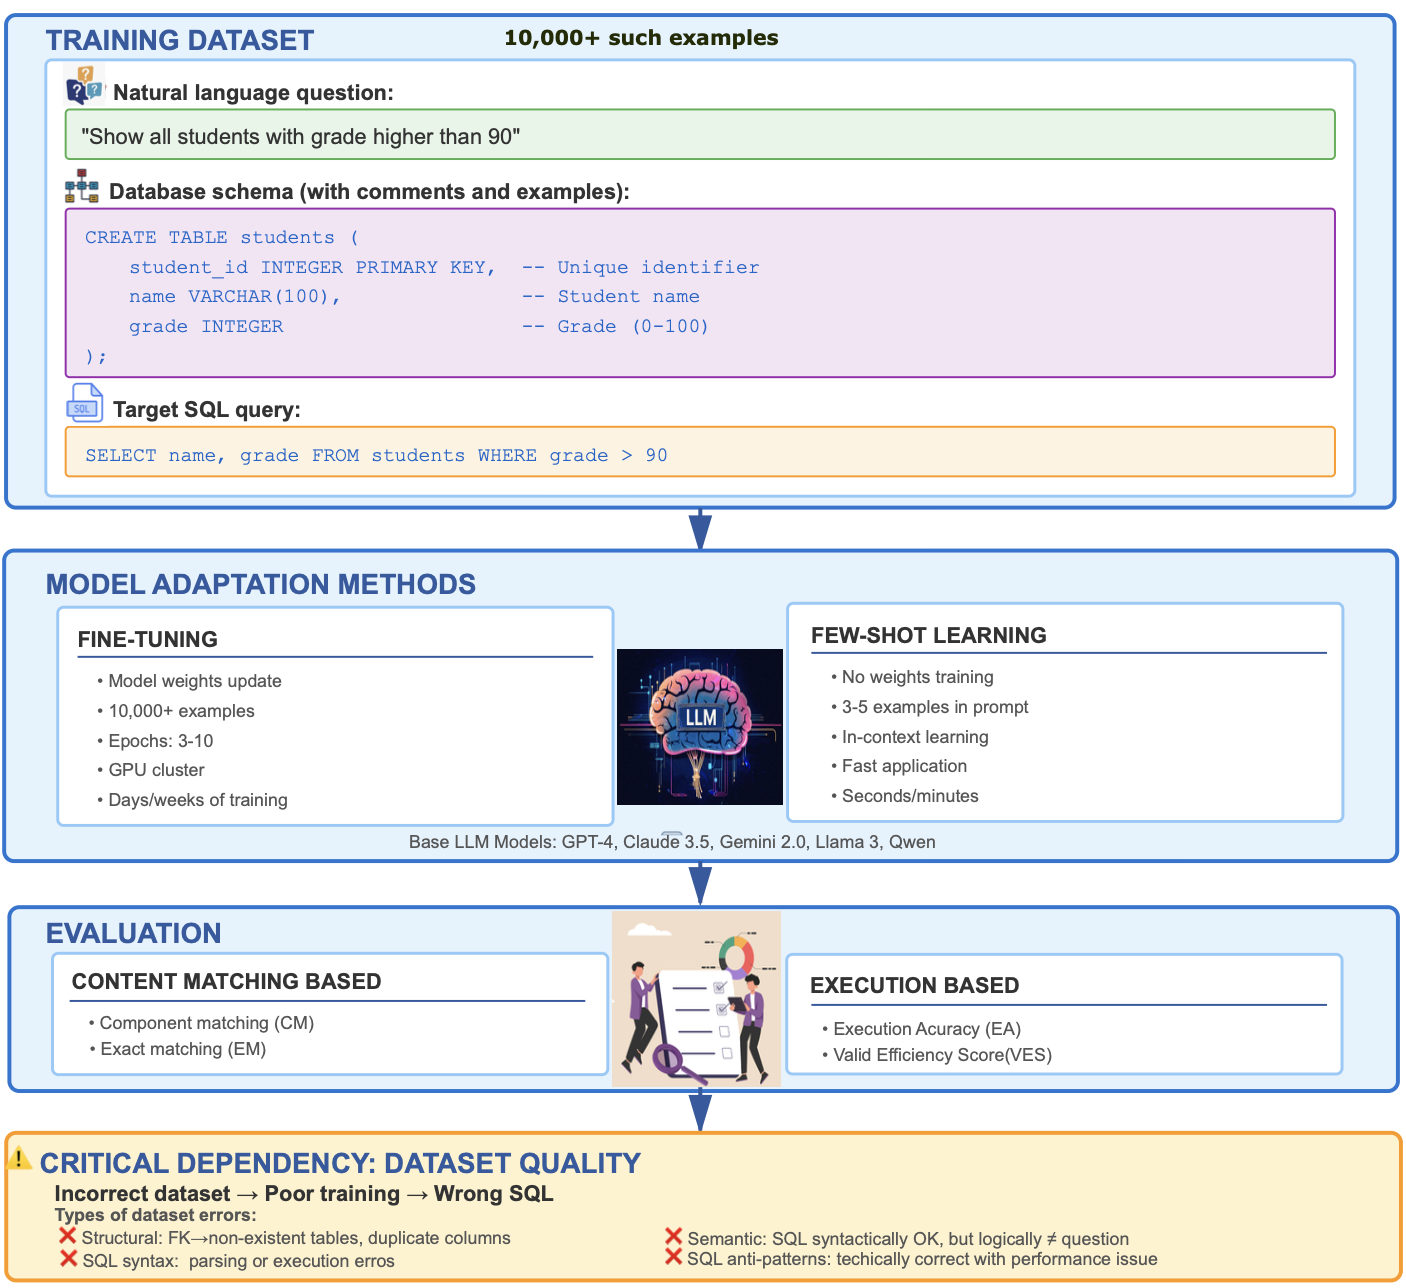
\includegraphics[width=0.8\textwidth]{figures/fig1_training_process.png}
  \caption{Complete training pipeline for LLMs in Text-to-SQL systems}
  \label{fig:training_process}
\end{figure}

From a practical standpoint, Text-to-SQL LLM systems are being actively deployed by leading cloud platforms. Snowflake Copilot can generate SQL from natural language in Snowsight~\cite{snowflake_copilot}; Databricks AI/BI Genie converts plain English questions into equivalent SQL queries~\cite{databricks_genie}; Microsoft Copilot in Fabric/Azure SQL supports Natural Language $\rightarrow$ SQL in SQL Database workspaces~\cite{microsoft_fabric_copilot}. This lowers the barrier for business analysts and non-technical users, providing data access without knowledge of SQL syntax.

The typical process of training LLMs for Text-to-SQL tasks includes three key components (Figure~\ref{fig:training_process}): a training dataset containing triplets of \{natural language question, database schema, Target SQL query\}, an adaptation method (fine-tuning or few-shot learning) and evaluation (content matching and execution based). During fine-tuning, models adjust their weights on large Text-to-SQL datasets to better capture the mapping between natural language and SQL. In few-shot settings, by contrast, the model relies on in-context learning, using only a handful of examples in the prompt without updating its parameters. In both cases, dataset quality is critical: in fine-tuning, even a small fraction of flawed examples among tens of thousands can introduce systematic errors, while in few-shot prompting each individual example directly shapes model behavior, so a single incorrect pair may lead to consistently wrong generations. Consider specific types of errors that may be present in datasets:

\begin{itemize}
\item \textbf{Database schema structural errors}: incorrect foreign keys (references to non-existent tables/columns), duplicate columns, multiple primary keys, unknown data types.
\item \textbf{SQL syntax errors}: queries that cannot be parsed or executed on corresponding databases.
\item \textbf{Semantic mismatches}: SQL queries that are syntactically correct but logically do not correspond to the natural language question (e.g., using SUM instead of AVG, incorrect JOIN conditions, missing necessary filters).
\item \textbf{SQL anti-patterns}: technically correct queries with performance or style issues (SELECT *, absence of LIMIT, functions in WHERE that block index usage).
\end{itemize}

\subsection*{Problem statement}
Despite the central role of datasets, most work on Text-to-SQL focuses on model architectures, prompting techniques and decoding strategies. The quality of popular benchmarks is typically assumed rather than measured. Existing analyses either provide high-level, descriptive statistics about datasets or focus on runtime validation of single generated queries instead of auditing entire corpora. Consequently, researchers and practitioners have limited visibility into structural defects, semantic mismatches or stylistic antipatterns hidden in widely used datasets. Therefore, our central research questions are:

\begin{itemize}
\item \textbf{RQ1}: How can we systematically assess the overall quality of Text-to-SQL datasets?
\item \textbf{RQ2}: How accurate and internally consistent are popular Text-to-SQL benchmarks that serve simultaneously as training and evaluation data?
\end{itemize}

\subsection*{Research objective}

This paper addresses this question by proposing a comprehensive validation framework for Text-to-SQL datasets and using Spider 1.0 as the primary end-to-end testbed for the framework. Our work is positioned within empirical software engineering: we treat benchmark datasets as software artefacts that should be inspected, measured and improved with the same rigour as source code or test suites.

\subsection*{Contribution statement}

The main contributions of this paper are:

\begin{enumerate}
\item A novel multi-layer validation architecture for Text-to-SQL datasets integrating schema validation, syntax analysis, execution testing, antipattern detection, and LLM-based semantic verification.
\item The first comprehensive empirical audit of all three Spider 1.0 partitions (11,840 examples total) across five complementary quality dimensions.
\item An open-source implementation of the validation framework, publicly available to enable reproducible quality assessment of existing and future Text-to-SQL benchmarks.
\item Concrete empirical evidence that widely-used benchmarks contain significant quality issues invisible to standard evaluation metrics, including concentrated referential integrity catastrophes, substantial schema heterogeneity, and systematic semantic ambiguities.
\end{enumerate}

\subsection*{How the paper is structured}

The rest of this paper is structured as follows: in~\Cref{sec:RelatedWork}, we briefly discuss work done in similar areas by other researchers; in~\Cref{sec:Methods}, we describe the architectural design and implementation of our validation framework; in~\Cref{sec:Results}, we report the results of applying the framework to Spider 1.0. Then, in~\Cref{sec:Discussion}, we discuss the collected results and threats to validity, and we conclude the paper in~\Cref{sec:Conclusions}.

\section{Related Work}\label{sec:RelatedWork}

We review prior work across three complementary dimensions: the evolution of Text-to-SQL benchmarks, empirical evidence on data quality's impact on model performance, and existing approaches to dataset quality assessment.

\subsection{Text-to-SQL Benchmarks and Datasets}

The development of Text-to-SQL systems has been fundamentally shaped by the evolution of benchmark datasets. Early large-scale efforts, particularly WikiSQL~\cite{zhong2017seq2sql}, provided a foundational testbed with 80,654 natural-language questions and corresponding SQL queries over 24,241 Wikipedia tables. While WikiSQL enabled initial data-driven experimentation at scale, its design imposed significant constraints: queries were limited to single tables with a restricted SQL grammar excluding JOINs, nested subqueries, and complex aggregations. These limitations hindered the evaluation of compositional reasoning and realistic multi-table relational scenarios.

The release of Spider~\cite{yu2018spider} at EMNLP 2018 marked a pivotal advancement in the field. Spider comprises 10,181 natural-language questions mapped to 5,693 unique SQL queries across 200 databases spanning 138 diverse domains. The dataset was meticulously constructed and validated by 11 Yale University students, ensuring rigorous annotation quality. A consolidated update published in 2020 resolved annotation inconsistencies and schema discrepancies, establishing the canonical Spider 1.0 version that remains the community standard. Spider's prominence derives from several key attributes: (1) systematic human validation ensuring semantic correctness, (2) balanced distribution across domains and difficulty levels, (3) realistic multi-table schemas with extensive foreign-key relationships reflecting real-world database design, and (4) comprehensive coverage of SQL constructs including nested queries, set operations, aggregation with grouping, and multi-hop reasoning patterns. As of 2025, Spider has become the most widely adopted benchmark in the field, with over 700 citations across major academic indexing services.

Complementary benchmarks have emerged to address specific evaluation dimensions not fully captured by Spider. The BIRD benchmark~\cite{li2023bird} targets large-scale, content-rich databases (approximately 33 GB total), introducing practical challenges such as noisy data values, complex entity resolution requirements, and external knowledge dependencies. BIRD provides 12,751 question--SQL pairs across 95 substantial databases covering 37 professional domains, making it particularly valuable for assessing system robustness under realistic production conditions with imperfect data quality and ambiguous terminology.

Synthetic data generation has emerged as a scalable approach to augment training corpora. Gretel's synthetic Text-to-SQL dataset~\cite{gretel_synth} (Gretel-Synth) offers over 100,000 high-quality examples spanning multiple business domains, while OmniSQL~\cite{omnisql} employs a multi-stage generation pipeline to produce more than 2.5 million training instances across 16,000+ synthetic databases, incorporating chain-of-thought reasoning annotations.

Despite the proliferation of alternative resources, Spider 1.0 remains the most comprehensive and widely adopted benchmark due to its unique combination of scale, structural diversity, annotation reliability, and faithful representation of relational complexity. However, even carefully curated benchmarks like Spider are not immune to annotation errors, ambiguous question formulations, or schema inconsistencies. The challenges are further amplified in synthetic datasets, where automated generation processes can introduce systematic biases and semantic inaccuracies at scale. These quality concerns underscore the critical need for robust, automated validation mechanisms capable of detecting and characterizing errors across diverse Text-to-SQL datasets.

\subsection{Data Quality and Robustness in Text-to-SQL}

Empirical evidence increasingly demonstrates that the quality of training and evaluation data has a direct and often nonlinear influence on the performance of Large Language Models (LLMs) in Text-to-SQL tasks.

The Dr.Spider study~\cite{drspider} provides one of the most rigorous analyses of this phenomenon. By applying controlled perturbations to questions, database schemas, and SQL queries, the authors showed that LLM performance degrades sharply under reduced data quality. On average, execution accuracy dropped by 14.0\%, and under the most severe perturbations the degradation reached 50.7\%, revealing that current models exhibit low robustness to inconsistencies or noise in the training and evaluation pipelines. Notably, errors involving schema semantics (e.g., incorrect foreign keys or column references) produced disproportionately large declines, underscoring the sensitivity of Text-to-SQL systems to structural dataset quality.

Complementary findings come from Snowflake's Arctic-Text2SQL study~\cite{arctic_text2sql}, which evaluated the effects of mixing high-quality benchmark data (Spider, BIRD) with various forms of synthetic data, including Gretel-Synth. The authors observed that introducing lower-quality or weakly aligned synthetic examples into training can reduce final model accuracy, even when the overall dataset size increases---highlighting an inverse scaling trend. Their ablation experiments showed that quality mismatches between datasets lead to unstable gradients, degraded reasoning traces, and incorrect operator selection in generated SQL queries. These results reinforce the observation that the benefits of larger datasets cannot compensate for inconsistencies, noise, or semantic drift in the data.

\subsection{Dataset Quality Assessment Frameworks}

Although dataset quality is critical for Text-to-SQL system performance, systematic validation methodologies remain limited. A recent contribution addressing this gap is the benchmark analysis framework proposed by Mitsopoulou and Koutrika~\cite{mitsopoulou2025analysis}. Their study characterizes Text-to-SQL datasets along three complementary dimensions: structural and operator diversity of SQL queries, schema size and complexity of associated databases, and lexical-syntactic properties of natural-language questions. This unified descriptive perspective provides valuable insight into dataset composition, differences across benchmarks, and how dataset properties relate to model error profiles. The authors further introduce an ``informative evaluation'' procedure that decomposes system errors into structural, operator, and variable mismatches, offering a more interpretable alternative to exact-match evaluation.

However, this analysis remains descriptive rather than diagnostic: it does not assess whether dataset entries are correct or semantically faithful. Several important aspects of dataset quality therefore fall outside its scope, including verification of schema integrity, checks of SQL syntactic and execution validity, and evaluation of semantic alignment between natural-language intent and SQL logic. Beyond surface-level schema linkage, the gold annotations are assumed to be correct, and no mechanisms are provided to detect mismatches between questions and queries. Moreover, the methodology is designed for aggregate statistics on existing benchmarks and does not scale to large modern datasets such as OmniSQL's 2.5M+ synthetic examples.

A complementary perspective is offered by Pandey et al.~\cite{pandey2024ensuring}, who propose a ``data accuracy'' validation framework for enterprise Text-to-SQL systems. Their approach focuses on runtime validation of generated SQL and query results through schema validation, syntax checking, logical consistency checks (e.g., aggregate--grouping coherence), data integrity verification, and multi-agent feedback loops implemented with LangGraph and AutoGen. Although this framework uses several components like those needed for dataset quality assurance, it is fundamentally designed for per-query validation in production systems rather than large-scale offline auditing of benchmark or synthetic corpora. It operates on individual generated queries and their results and therefore does not analyze dataset-level error patterns, measure overall ``dataset health'', or provide tooling for systematic dataset curation. Moreover, the framework is presented primarily at an architectural and conceptual level: there is no publicly available implementation, no quantitative evaluation on standard benchmarks (e.g., Spider, BIRD, OmniSQL), and no support for batch-mode processing of tens of thousands of NL--SQL pairs. Semantic checks are restricted to intra-SQL consistency (e.g., aggregates vs. GROUP BY) and do not address the correctness of the natural-language--to-SQL mapping across an entire dataset.

Additional efforts in the literature acknowledge the importance of validation but remain fragmented and narrowly scoped. Synthetic data pipelines (e.g., Gretel, OmniSQL) typically apply internal LLM-based or heuristic filters, while many works rely almost exclusively on execution-based filtering---discarding examples whose SQL fails to run on the corresponding database. Although such filtering can improve training stability, it is ultimately naïve and insufficient: successful execution does not verify the correctness of SQL logic, the semantic alignment between the question and the query, the integrity of the underlying schema, or the presence of stylistic and efficiency-related anti-patterns. Consequently, these procedures cannot serve as general-purpose dataset auditing methods and address only a small subset of the quality issues that arise in modern Text-to-SQL datasets.

Taken together, existing approaches provide important analytical foundations and illustrate the need for quality control, but they do not offer a comprehensive, automated, and scalable solution for validating Text-to-SQL datasets themselves. Our work builds on these insights by introducing a multi-level validation framework---covering structural, syntactic, semantic, and stylistic dimensions---implemented in an extensible open-source system designed to evaluate both human-curated benchmarks and large-scale synthetic datasets at scale.

\section{Methods}\label{sec:Methods}

In this section, we describe the design, architecture, and implementation of our comprehensive Text-to-SQL dataset validation framework.

\subsection{Architectural overview of the text2sql-dataset-analyzer framework}

In this section we present \texttt{text2sql-dataset-analyzer}, a novel framework and, to the best of our knowledge, the first dedicated tool for systematic, multi-layer quality assessment of Text-to-SQL benchmarks. The framework is released as open-source software, which allows other researchers and practitioners to inspect, extend, and apply it to their own Text-to-SQL corpora.

\textbf{Design principles.} The system represents a streaming data-processing architecture designed to address the challenges of large-scale Text-to-SQL dataset validation and quality assessment. The architecture implements three foundational design principles: modularity through protocol-based component interfaces, scalability via constant-memory streaming processing, and extensibility through automatic dependency injection. This design enables the system to process datasets of arbitrary size while maintaining deterministic memory footprint characteristics, a critical requirement when analyzing multi-gigabyte benchmark datasets such as Spider, BIRD, or OmniSQL 2.5 M.

\textbf{Technology Stack.} The implementation relies on a carefully selected technology stack centered on Python 3.11~\cite{python311}, chosen for its mature ecosystem of SQL tooling and support for large language model integration. DuckDB~\cite{duckdb} serves as the primary analytics backend, offering columnar storage optimized for analytical queries while exposing a standard SQL interface. For interaction with relational databases, we use SQLAlchemy 2.0~\cite{sqlalchemy}-based adapters, which provide a uniform abstraction layer over concrete engines; in the current implementation, SQLite and PostgreSQL are supported as execution backends, but additional engines can be integrated with minimal effort. SQL parsing and structural analysis are handled by sqlglot~\cite{sqlglot}, a dialect-aware parser capable of dealing with syntactic variations across SQLite, PostgreSQL, MySQL, and other SQL dialects commonly encountered in Text-to-SQL datasets. Component orchestration relies on the \texttt{dependency\_injector} library~\cite{dependency_injector}, which facilitates type-safe dependency resolution and enables runtime composition of analysis pipelines through declarative YAML configuration loaded via PyYAML~\cite{pyyaml}.

\textbf{User Interface.} User interaction with the system occurs primarily through a command-line interface exposed via the \texttt{text2sql} entry point. The interface supports two distinct operational modes corresponding to the system's primary use cases. The first mode, invoked through \texttt{text2sql run --config <config.yaml>}, executes the complete analysis pipeline from raw dataset ingestion through all configured analyzers to final metric persistence and report generation. The second mode, accessible via \texttt{text2sql report}, enables standalone report generation from previously computed metrics, supporting both configuration-driven batch report generation (\texttt{--config}) and targeted single-report generation (\texttt{--database <path> --type <report-type>}). This separation of concerns between analysis and reporting allows researchers to iterate on report designs and formats without re-executing computationally expensive analysis stages, particularly relevant when semantic validation via large language models can require hours of processing time.

\subsection{Five-Layer System Architecture}

The system architecture follows a layered design pattern comprising five distinct layers, each responsible for a specific aspect of the data processing pipeline (Figure~\ref{fig:architecture}). This layered organization promotes separation of concerns, facilitates independent testing and development of components, and enables selective activation or deactivation of functionality based on analysis requirements.

\begin{figure}[htbp]
  \centering
  
\includegraphics[width=0.9\textwidth]{figures/fig2_architecture.png}
  \caption{Five-layer architecture of the text2sql-pipeline system}
  \label{fig:architecture}
\end{figure}

\textbf{Input Layer.} The Input Layer abstracts heterogeneous data sources behind a common iterator interface. It implements four specialized loaders tailored to data formats prevalent in Text-to-SQL research. The JSONL Loader provides streaming access to line-delimited JSON files, including gzip-compressed variants. The CSV Loader supports delimiter detection and encoding inference to handle noisy, real-world CSV files. Standard JSON arrays are handled by the JSON Loader, and the HuggingFace Loader connects directly to the HuggingFace Datasets Hub, avoiding manual download and reformatting. All loaders implement Python's iterator protocol and yield records on demand, keeping memory usage essentially constant with respect to dataset size.

\textbf{Normalization Layer.} The Normalization Layer standardizes records originating from diverse datasets through three sequential normalizers. The Alias Mapper reconciles different field names (e.g., \texttt{query} vs \texttt{sql}, \texttt{db\_id} vs \texttt{dbId}) into a canonical schema. The ID Assignment component guarantees a unique identifier for each record using either counters or content-based hashes, supporting consistent cross-referencing between the annotated dataset and the metrics database. The DB Identity Normalizer ensures that each record is linked to a valid database: it validates provided database identifiers or, when necessary, builds databases from embedded DDL schemas and derives stable IDs from schema hashes. The result is a normalized DataItem with mandatory fields (\texttt{id}, \texttt{question}, \texttt{sql}, \texttt{dbId}), an optional schema, and a metadata dictionary.

\textbf{Analysis Layer.} The Analysis Layer is the computational core, hosting five analyzers that cover complementary quality dimensions of Text-to-SQL data:

\begin{enumerate}
\item \textbf{Schema Validation Analyzer} checks database integrity, including several classes of foreign-key violations, case-insensitive column name duplicates, and type compatibility with the target SQL dialect. A DB-ID-based cache reuses schema introspection results across queries sharing the same database.

\item \textbf{Query Syntax Analyzer} performs static analysis using the sqlglot parser. It builds abstract syntax trees, derives normalized complexity scores on a 0--100 scale based on SQL constructs and nesting depth, extracts structural features (e.g., JOIN counts, subquery depth, CTEs, aggregations, window functions), and assigns difficulty labels (Easy, Medium, Hard, Expert).

\item \textbf{Query Execution Analyzer} evaluates dynamic executability within the corresponding database. Queries are run in a sandboxed, SELECT-only mode; execution time and row counts are recorded, and failures are categorized to distinguish syntax problems, semantic errors, and connectivity issues.

\item \textbf{Query Antipattern Detector} uses a rule-based approach to flag 14 common SQL antipatterns, such as missing LIMIT clauses, SELECT *, functions in WHERE predicates blocking index usage, correlated subqueries with quadratic complexity, and implicit joins. Each antipattern contributes a weighted penalty to a 0--100 quality score.

\item \textbf{Semantic LLM Judge Analyzer} uses large language models to assess how well SQL queries answer their natural-language questions.
\end{enumerate}

\textbf{Output Layer.} The Output Layer persists analysis results via two complementary streams. The Annotated Dataset augments each original record with all analyzer metadata and stores it in JSONL format, preserving a detailed provenance for downstream filtering or model training. In parallel, the DuckDB Analytics Database stores structured metrics in a columnar OLAP database. Users can query it with SQL, export results to Pandas or Polars, or write Parquet files for long-term storage and integration with external analytics workflows. This dual strategy preserves both record-level detail and dataset-level statistics without re-running the pipeline.

\textbf{Report Generation Layer (optional).} The Report Generation Layer converts metrics stored in DuckDB into human-readable Markdown reports. Controlled via a \texttt{reports.enabled} flag, it can be disabled during rapid experimentation on large datasets. When active, it produces seven report types: overall summary statistics; schema validation issues; semantic validation problems (queries judged incorrect or unanswerable); execution failures; structural complexity and difficulty distributions; table coverage analysis; and SQL quality assessments based on antipatterns. Because DuckDB is the single source of truth for metrics, reports can be regenerated or customized at any time via ad-hoc SQL queries, and report generation can be omitted entirely when performance constraints are critical.

\subsection{Data Flow and Processing Model}

Figure~\ref{fig:dataflow} shows the lifecycle of a single dataset record as it moves through the streaming pipeline. The system follows the iterator pattern: each record is processed end-to-end before the next one is loaded, without ever holding the full dataset in memory. Processing starts when a loader reads a raw record and yields it as a Python dictionary. The record then passes through the three normalizers described earlier. Each normalizer applies its transformation or validation and forwards the result, producing a standardized DataItem with all required fields present and a verified database identity. The normalized DataItem then enters the analysis pipeline, implemented as a chain of generator-based analyzers. Each analyzer consumes a DataItem, runs its logic (schema validation, syntax analysis, execution testing, antipattern detection, or semantic judging), writes metrics to DuckDB, enriches the DataItem's metadata, and yields it to the next analyzer. All configured analyses for one record complete before the next record is read, preserving strict streaming semantics. After the final analyzer, the fully annotated DataItem reaches the output layer. One branch serializes it to a JSONL file that contains the original fields plus all metadata, enabling downstream use without access to the metrics database. The other branch accumulates structured metrics in DuckDB with batched writes, supporting efficient aggregate analysis.

\begin{figure}[htbp]
  \centering
  
\includegraphics[width=0.85\textwidth]{figures/fig3_dataflow.png}
  \caption{Data flow through the pipeline from input to output}
  \label{fig:dataflow}
\end{figure}

The last report layer, which can be disabled via configuration (\texttt{reports.enabled = false}), reads metrics from DuckDB and produces seven types of human-readable analytical reports in Markdown format.

\subsection{Database Identity Normalization Algorithm}\label{sec:dbidentity}

The Database Identity Normalizer addresses a fundamental challenge in Text-to-SQL dataset processing: ensuring that every record can be associated with a valid, accessible database instance against which SQL queries can be validated and executed. This challenge arises from the diversity of dataset formats and conventions employed across the Text-to-SQL research community, where some datasets provide explicit database identifiers referencing pre-existing database files (Spider and Bird datasets), others include DDL schemas allowing dynamic database construction, and some provide both, occasionally with inconsistencies between the identifier and schema.

\begin{figure}[htbp]
  \centering
  
\includegraphics[width=0.75\textwidth]{figures/fig4_dbidentity.png}
  \caption{DbIdentity normalization process: guaranteed dbId filling via health check or creation from DDL}
  \label{fig:dbidentity}
\end{figure}

The algorithm implements a decision tree with three primary branches corresponding to different combinations of database identifier presence and schema availability (Figure~\ref{fig:dbidentity}).

In the first scenario, when a record provides an explicit database identifier, the normalizer invokes a health check through the database manager, querying whether the referenced database exists and contains data. If the check passes, the record proceeds unchanged; if it fails, the normalizer attempts to recreate the database from its stored DDL schema.

The second scenario handles records lacking explicit database identifiers but including DDL schema specifications, a pattern commonly encountered in synthetic datasets or benchmark subsets designed for testing schema understanding capabilities. For these records, the normalizer computes a cryptographic hash (SHA-256) of the DDL schema text, generating a deterministic identifier that remains consistent across multiple pipeline executions processing the same schema. The normalizer then checks whether a database with this computed identifier already exists; if so, it reuses that database instance, leveraging caching to avoid redundant database creation operations when multiple records share identical schemas. If no such database exists, the normalizer creates a new database from the DDL schema, assigns it the computed hash identifier, and populates the record's \texttt{dbId} field with this identifier. This deterministic identifier generation strategy ensures reproducibility while supporting the analysis of DDL-only datasets that lack pre-existing database files.

The third scenario represents failure cases where records provide neither a database identifier nor a DDL schema. In this situation, the normalizer raises a \texttt{ValueError} with a descriptive error message, immediately halting processing of that record. This fail-fast behavior reflects a deliberate design decision: rather than attempting graceful degradation by skipping validation steps that require database access, the system treats the absence of database identification as a fatal data quality issue that must be addressed at the source. This strict validation ensures that downstream analyzers can rely on the guaranteed presence of a valid database identifier, simplifying their implementation and preventing silent failures where analyses would be skipped due to missing database access.

\subsection{Multi-Model Semantic Validation Architecture}\label{sec:semantic}

The Semantic LLM Judge Analyzer constitutes the most sophisticated component of our validation pipeline, employing large language models to assess whether SQL queries correctly answer their associated natural language questions. This semantic validation capability addresses a critical limitation in traditional formal validation approaches: while syntax checking and execution testing verify technical correctness, only semantic analysis can determine whether a syntactically valid, successfully executing query implements the intended meaning of the natural language question. Our analyzer implements this capability through a four-stage pipeline (Figure~\ref{fig:semantic_judge}) combining intelligent context generation, prompt engineering, multi-model consensus voting, and result aggregation.
\begin{figure}[htbp]
    \centering
    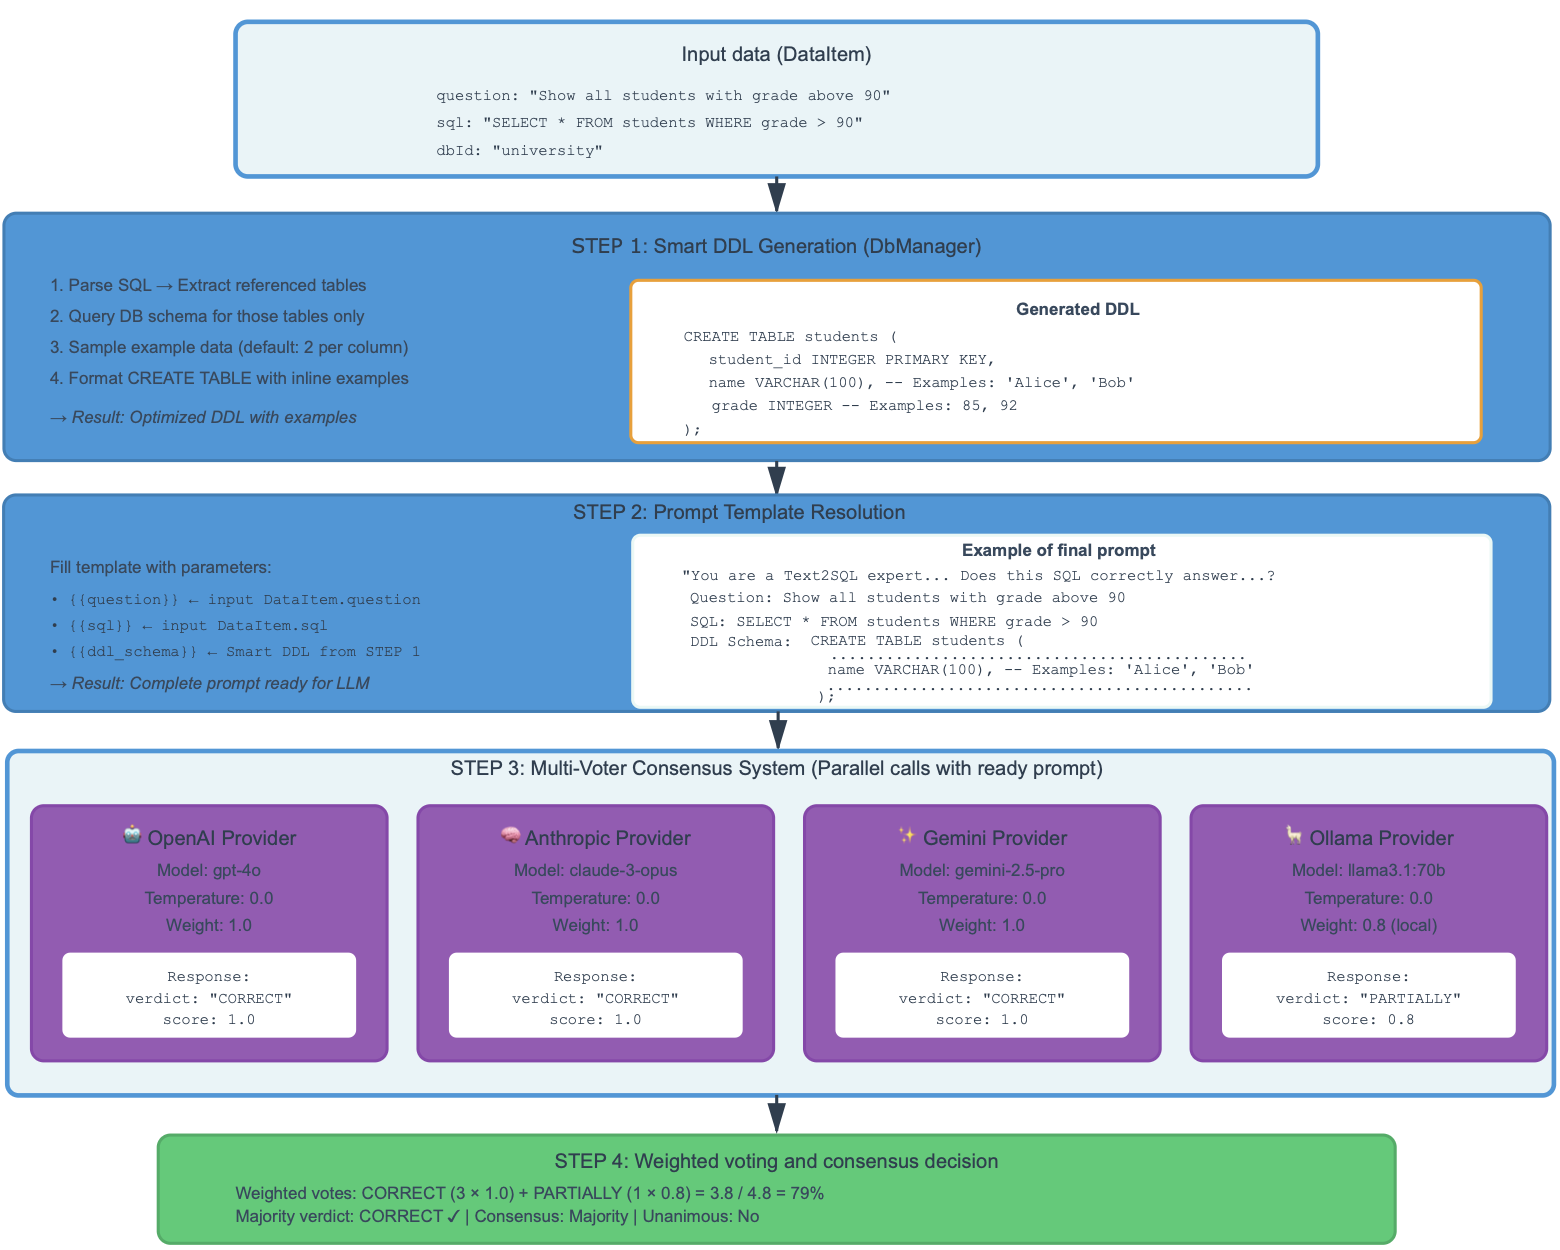
\includegraphics[width=0.8\textwidth]{figures/fig5_semantic_judge.png}
    \caption{Architecture of the Semantic LLM Judge with multi-model consensus voting}
    \label{fig:semantic_judge}
  \end{figure}
  
\textbf{Smart DDL Generation.} The first stage addresses the token efficiency challenge inherent in providing database schema context to language models. Naïvely transmitting complete database schemas can consume thousands of tokens for databases with dozens of tables, rapidly exceeding context window limits or consuming substantial portions of available context that could be better utilized for reasoning. The smart generation algorithm mitigates this issue through a multi-step optimization process. First, the system parses the SQL query using sqlglot to construct an abstract syntax tree, from which it extracts the set of tables explicitly referenced in FROM clauses, JOIN specifications, and subqueries. Second, the database adapter queries the system catalog (\texttt{sqlite\_master} for SQLite, \texttt{information\_schema} for PostgreSQL) to retrieve metadata only for these referenced tables, including column names, data types, primary keys, and foreign key relationships. Third, the system executes SELECT queries to sample a configurable number of example values from each column (defaulting to 2 examples per column), providing concrete data instances that help language models understand the semantic content of columns beyond what data type information conveys.

Finally, the collected metadata is formatted into CREATE TABLE statements with inline comments containing the example values, producing a minimal DDL specification that includes only information relevant to the query under analysis. This optimization typically reduces token consumption by factors of 5-10 compared to full schema transmission while preserving the contextual information that language models require for accurate semantic reasoning.

\textbf{Prompt Template Resolution.} The second stage combines the generated smart DDL with contextual elements to produce complete evaluation prompts. Templates are loaded from YAML configuration files to facilitate experimentation with different prompt formulations. Each template contains dynamic placeholders:

\begin{itemize}
\item \texttt{\{\{question\}\}}: The natural language question from the dataset, providing ground truth for query semantics
\item \texttt{\{\{sql\}\}}: The SQL query under evaluation, formatted with syntax highlighting and normalized whitespace
\item \texttt{\{\{ddl\_schema\}\}}: The smart DDL from Stage 1, supplying necessary schema context
\item \texttt{\{\{dialect\}\}}: Optional SQL dialect specification (sqlite, postgresql, etc.) for correct interpretation of dialect-specific syntax
\end{itemize}

The assembled prompt specifies a strictly structured response format in which the model must return a single JSON object with exactly two keys, ``verdict'' and ``explanation'' (Figure~\ref{fig:prompt_structure}). The ``verdict'' field is constrained to one of four categorical labels: CORRECT (the query fully and accurately answers the question with no semantic issues), PARTIALLY\_CORRECT (the query is mostly correct but exhibits minor deficiencies such as missing DISTINCT clauses when duplicates are possible, imprecise date/time boundaries, NULL-handling edge cases, or non-deterministic GROUP BY selections that do not fundamentally invalidate the result), INCORRECT (the query contains fundamental semantic errors including wrong table or column selections, missing or incorrect JOIN conditions, flawed aggregation logic, or erroneous WHERE clause predicates that produce fundamentally incorrect results), and UNANSWERABLE (the question cannot be answered from the provided schema due to missing tables or columns, requirements for external data not present in the database, or inherent ambiguity or contradictions in the question itself).

\begin{figure}[htbp]
  \centering
  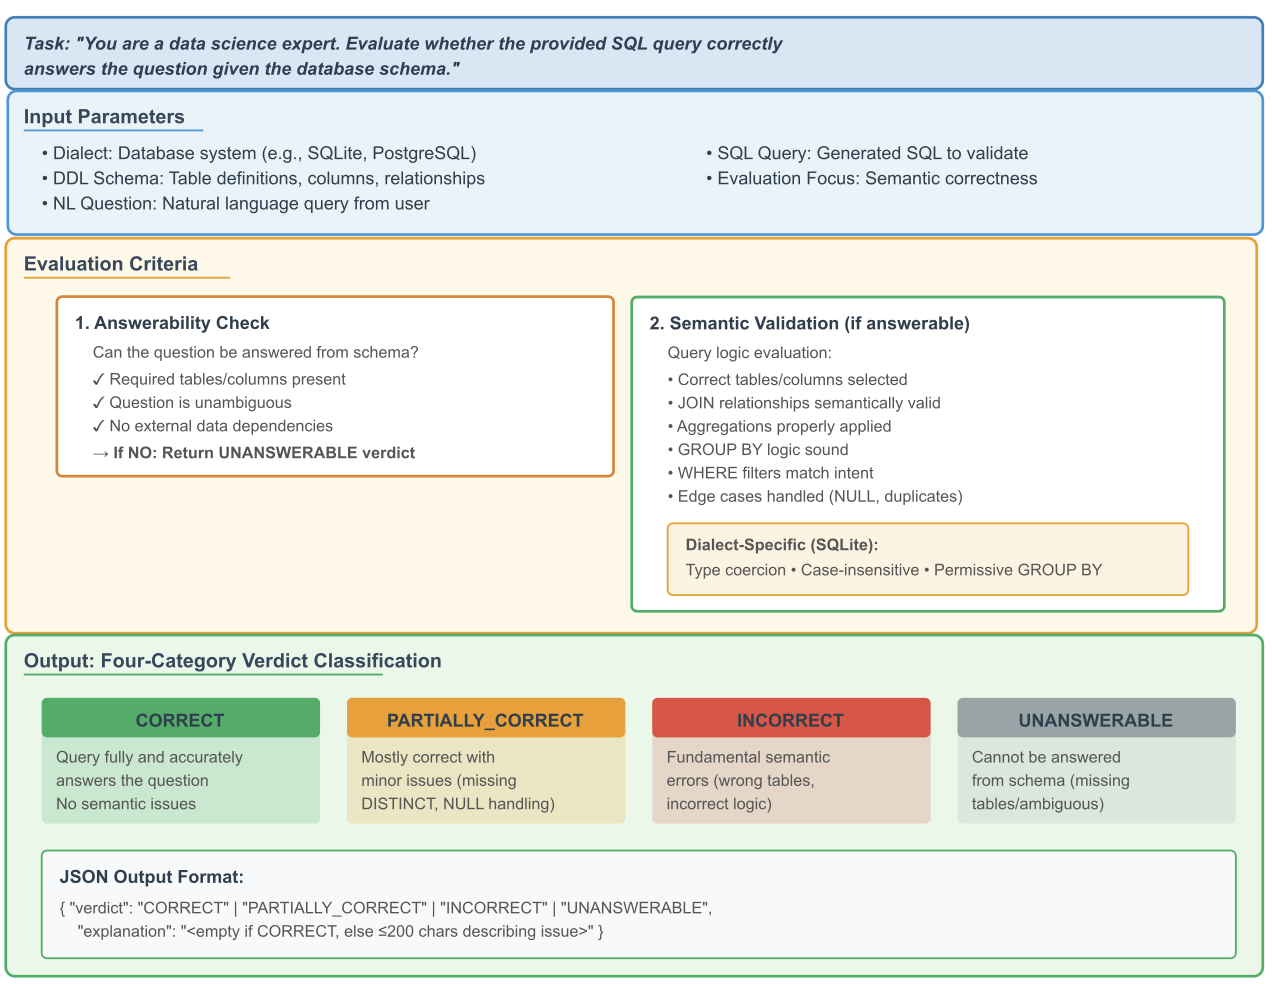
\includegraphics[width=0.85\textwidth]{figures/fig7_prompt.png}
  \caption{LLM prompt structure with input parameters, evaluation criteria, and four-category verdict classification}
  \label{fig:prompt_structure}
\end{figure}

The ``explanation'' field encodes a short natural-language justification; for CORRECT verdicts, the explanation is required to be an empty string, thereby preventing spurious narrative output, while for all other verdicts, the explanation must be a concise single-line description (bounded to at most 160--200 characters) that identifies the dominant semantic issue. This response specification transforms otherwise free-form LLM outputs into machine-parseable judgments that can be aggregated systematically across large datasets.

\textbf{Multi-Model Consensus Voting.} This stage queries multiple language models in parallel, collecting independent judgments. Our architecture supports four provider categories, each offering distinct characteristics:

\begin{itemize}
\item \textbf{OpenAI models} (GPT-5, GPT-4o, etc.) provide strong reasoning capabilities and reliable structured output generation, though with relatively high per-token costs.
\item \textbf{Anthropic models} (Claude-4.5-sonnet, Claude-3-sonnet, etc.) offer alternative reasoning approaches that often exhibit different error patterns from GPT models, valuable for identifying edge cases where consensus breaks down.
\item \textbf{Google models} (Gemini-2.5-pro, Gemini-1.5-pro, etc.) deliver competitive performance with distinct training data and architectural choices that surface different perspectives on ambiguous cases.
\item \textbf{Ollama models} (Llama-3.1-70b, Mistral, Mixtral, etc.) enable fully local execution without API costs or rate limits, though typically with reduced accuracy compared to frontier commercial models.
\end{itemize}

This multi-model approach provides natural defense against systematic biases of individual models, where inter-model agreement serves as a reliability indicator for downstream analysis.

\textbf{Consensus decision.} The fourth stage aggregates the individual model responses through weighted voting to determine consensus verdicts and identify cases requiring human review. Each model is associated with a non-negative scalar weight specified in the configuration file, allowing researchers to encode prior beliefs about the relative reliability or cost-effectiveness of different providers (for example, assigning higher weights to empirically validated frontier models while giving lower weights to cheaper or fully local models). The aggregation procedure operates along two complementary axes. First, it computes an unweighted majority verdict by counting, for each of the four categories, how many models produced that verdict; a majority consensus is deemed to exist when a single category accounts for more than half of all non-failed model responses, and a verdict is unanimous when all such responses coincide. Second, it derives a scalar semantic quality score in the closed interval $[0,1]$ by mapping CORRECT to 1.0, PARTIALLY\_CORRECT to 0.5, and both INCORRECT and UNANSWERABLE to 0.0, and then computing a provider-weighted average according to formula:

\begin{equation}
\text{score}_{\text{consensus}} = \frac{\sum_{i=1}^{n} w_i \cdot v_i}{\sum_{i=1}^{n} w_i}
\end{equation}

where $v_i$ denotes the mapped verdict value and $w_i$ the corresponding model weight. This score captures the aggregate tendency of weighted models to regard a query as semantically adequate, while the majority and unanimity indicators characterize the degree of inter-model agreement. Records lacking any strict majority or exhibiting strongly divergent verdicts across models are of particular interest for dataset curation, as they frequently correspond to questions whose intent is underspecified, to SQL queries with subtle semantic flaws, or to cases where multiple, mutually incompatible interpretations of the question are plausible.

The multi-model semantic validation architecture addresses several research challenges in Text-to-SQL evaluation. By employing multiple models with different architectures and training data, the system reduces the risk of systematic biases that might arise from relying on a single model family. The consensus voting mechanism provides natural uncertainty quantification, with disagreement among models serving as a signal that examples may be problematic or ambiguous rather than clearly correct or incorrect. The structured output format with confidence scores enables downstream analysis to weight semantic validation results appropriately, for example by flagging low-confidence verdicts for human review or by analyzing whether certain query patterns systematically produce low-confidence judgments.

\subsection{Protocol-Based Architecture and Dependency Injection}

The system architecture employs Python's Protocol typing construct to establish clear contracts between components while maintaining loose coupling between interface definitions and their concrete implementations.

\begin{figure}[htbp]
  \centering
  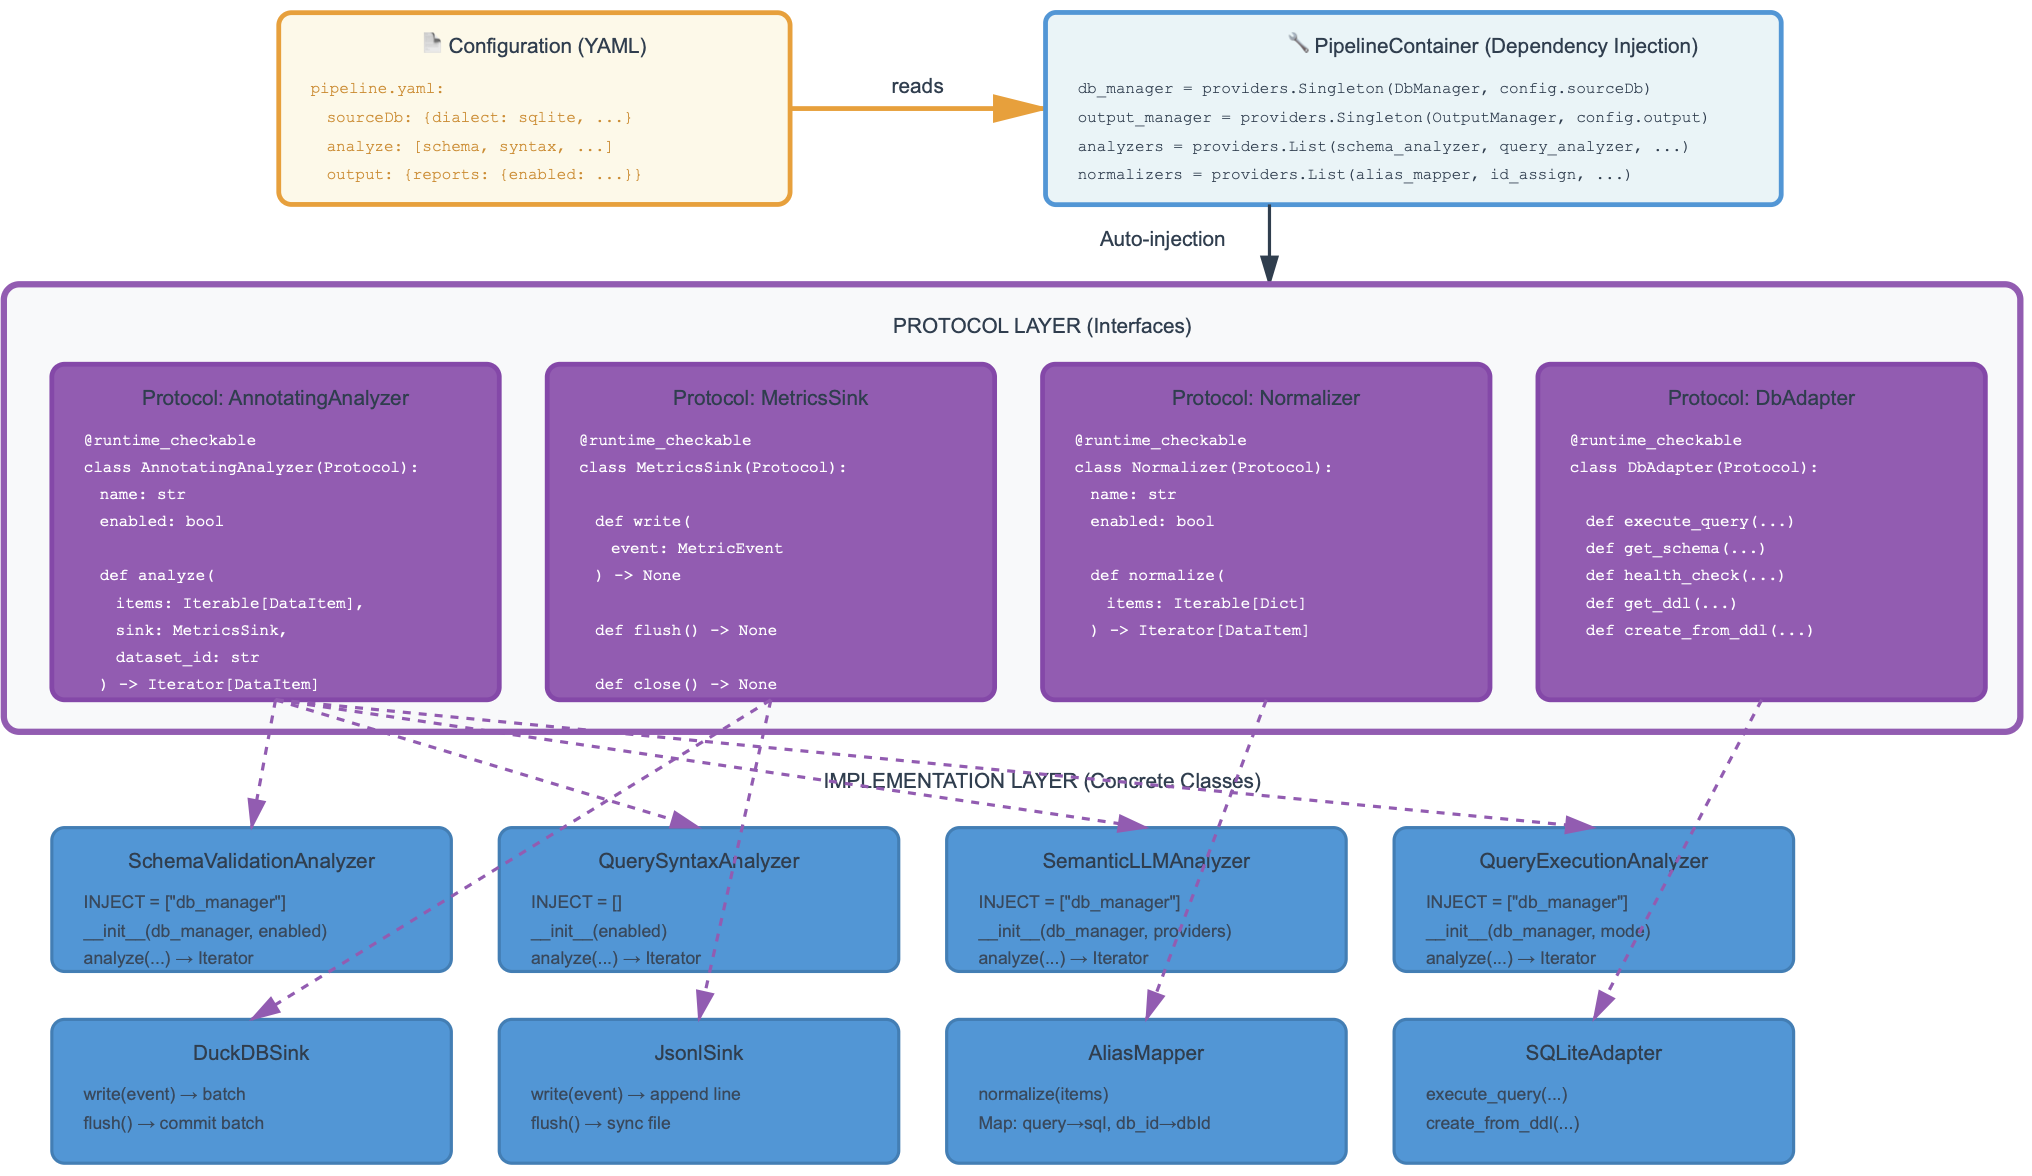
\includegraphics[width=0.8\textwidth]{figures/fig8_protocols.png}
  \caption{Protocol-based architecture with automatic dependency injection}
  \label{fig:protocols}
\end{figure}

This architectural pattern, analogous to interface-based programming in statically typed languages, provides the benefits of explicit type checking and interface documentation while preserving the flexibility and rapid iteration characteristics of dynamic Python development (Figure~\ref{fig:protocols}).

The \textbf{AnnotatingAnalyzer Protocol} defines the essential contract that all analyzer implementations must satisfy, specifying required attributes including a string-valued name identifier and a boolean enabled flag for runtime toggling.

The \textbf{MetricsSink Protocol} abstracts the mechanisms through which analyzers persist their computed metrics, defining three essential operations: write for accepting individual metric events, flush for ensuring durable persistence, and close for cleanup.

The \textbf{Normalizer Protocol} specifies the interface for components responsible for data standardization, requiring a normalize method that accepts an iterable of raw dictionary objects and returns an iterable of validated, enriched records.

The \textbf{DbAdapter Protocol} encapsulates dialect-specific database operations, defining methods for query execution with configurable safety modes, schema introspection for retrieving table and column metadata, and connection lifecycle management.

Component orchestration within the protocol-based architecture relies on the \texttt{dependency\_injector} library to automate the complex wiring of object graphs that arise from interdependent components. Each layer's components are registered in a declarative container specification, with dependencies expressed through type annotations.

The protocol-based architecture with dependency injection offers several significant advantages for research software development. The explicit protocol interfaces serve as machine-checkable documentation, automated dependency resolution eliminates manual wiring complexity, and the loose coupling between protocols and implementations facilitates testing through mock implementations.

\section{Experimental Setup and Results}\label{sec:Results}

We present the results of applying our validation framework to all three partitions of the Spider 1.0 benchmark, analyzing 11,840 examples across five quality dimensions.

\subsection{Experimental Methodology}

We select Spider 1.0 dataset as our primary test dataset because it has become the most widely used benchmark for both training and evaluating Text-to-SQL models in the research community. Its ubiquitous adoption as the standard evaluation framework---reflected in countless publications and model leaderboards since 2018---means that any quality issues, ambiguous examples, or annotation errors we identify in Spider have direct implications for the validity of results reported across numerous studies that rely on this benchmark.

The experimental methodology employs comprehensive multi-layer validation across all three Spider partitions (test, dev, train) to assess both overall dataset quality and consistency characteristics between partitions. This comparative approach enables detection of systematic differences that might affect the reliability of training and evaluation procedures, a consideration particularly important given that many published Text-to-SQL systems report performance metrics only on the test partition while using dev for hyperparameter tuning.

The three analyzed partitions exhibit substantially different scales: Spider Test contains 2,147 examples spanning 40 unique databases, Spider Dev includes 1,034 examples across 20 databases, and Spider Train comprises 8,659 examples distributed over 146 databases. This size disparity introduces methodological considerations for certain analyses, particularly semantic validation via large language models, where the computational cost scales linearly with dataset size and where processing all 8,659 training examples would incur API costs exceeding \$200-320 at current pricing.

All analyses employed SQLite as the target SQL dialect, matching Spider's native database format. The pipeline activated all five analyzers for all three partitions. The LLM configuration utilized Gemini 2.5 Pro and GPT-5 as voting models, both configured with temperature=0.0 to maximize determinism and weight=1.0 to ensure equal voting power, employing majority consensus for verdict determination. The DDL generation mode operated in \texttt{query\_derived} mode, extracting only tables referenced in each SQL query rather than transmitting complete database schemas, reducing token consumption.

Processing time varied substantially between partitions due to both dataset size and LLM API latency. Spider Test required approximately 12.7 hours when including LLM-based semantic validation, Spider Dev consumed roughly 6.1 hours under identical configuration, while Spider Train required approximately 49 hours to complete full semantic validation across all 8,659 examples. The LLM API latency and inference time typically requires 2-10 seconds per record compared to 50-100 milliseconds for the combined execution of all formal analyzers, explaining the domination of overall runtime by semantic validation. The decision to proceed with complete LLM validation across all partitions, despite the substantial computational investment, enables unprecedented comprehensive semantic quality assessment covering all 11,840 Spider examples rather than relying on sampling or limiting analysis to the smaller test partitions.

\subsection{Database Schema Integrity Assessment}

Schema integrity validation examines the structural correctness of database definitions, detecting errors that could prevent successful query execution even for syntactically valid SQL statements. Table~\ref{tab:schema_overall} presents aggregate schema validation metrics across all three Spider partitions.

\begin{table}[ht]
    \caption{Comparative database schema validation results across Spider partitions}
    \label{tab:schema_overall}
    \centering
    \footnotesize
    \begin{tabular}{lcccc}
        \toprule
        \textbf{Metric} & \textbf{Spider Test} & \textbf{Spider Dev} & \textbf{Spider Train} & \textbf{Best} \\
        \midrule
        Total databases & 40 & 20 & 146 & -- \\
        Valid databases & 36 (90.0\%) & 13 (65.0\%) & 114 (78.1\%) & Test \\
        Invalid databases & 4 (10.0\%) & 7 (35.0\%) & 32 (21.9\%) & Test \\
        Total schema errors & 10 & 21 & 58 & Test \\
        Databases with FK violations & 4 & 7 & 27 & Test \\
        Total FK integrity violations & 0 & 2,400 & 38,273 & Test \\
        \bottomrule
    \end{tabular}
\end{table}

The results reveal a clear quality gradient across partitions, with Test achieving 90.0\% schema validity, substantially exceeding Train at 78.1\% and Dev at 65.0\%. This ordering contradicts the intuitive expectation that training data should exhibit higher quality than test data.

Analysis of error type distribution (Table~\ref{tab:schema_errors}) identifies dominant patterns contributing to schema invalidity. Foreign Key Type Mismatch errors, where referencing and referenced columns possess incompatible data types, constitute 39.1\% of all detected issues (34 of 89 total errors).

\begin{table}[ht]
    \caption{Distribution of schema error types across partitions}
    \label{tab:schema_errors}
    \centering
    \footnotesize
    \begin{tabular}{lccc}
        \toprule
        \textbf{Error Type} & \textbf{Spider Test} & \textbf{Spider Dev} & \textbf{Spider Train} \\
        \midrule
        Foreign Key Type Mismatch & 0 & 0 & 34 \\
        Foreign Key Target Not Found & 8 & 12 & 21 \\
        Duplicate Column Names & 2 & 9 & 3 \\
        \bottomrule
    \end{tabular}
\end{table}

A particularly concerning finding emerges from analysis of foreign key data integrity violations, distinct from the structural foreign key errors discussed above. While 10 databases across all partitions contain referential integrity violations, the distribution is highly skewed: sakila\_1 (Train) contains 38,273 violations and flight\_2 (Dev) contains 2,400 violations, together accounting for 99.5\% of all referential integrity problems. These data-level violations occur when foreign key values in child tables reference non-existent primary key values in parent tables, breaking relational integrity assumptions. For example, the sakila\_1 database's film\_actor junction table references film and actor IDs that do not exist in the parent tables, making it impossible to correctly execute queries requiring joins between these tables. The flight\_2 violations similarly corrupt the relationships between flights, airlines, and airports, creating scenarios where SQL queries that attempt to join these tables will either fail or produce incomplete result sets missing records with dangling references. Such integrity violations not only invalidate queries in the benchmark but also undermine any model training on these examples, as models may learn incorrect patterns from corrupted joins.

The Train partition exhibits an additional quality issue absent from Test and Dev: 41 tables across 4 databases (academic, imdb, yelp, restaurants) contain schema definitions but no data rows, representing empty tables that cannot support meaningful query evaluation. For instance, the \texttt{academic} database includes empty tables for conference proceedings and citations, preventing execution of queries that reference those tables. Similarly, the large-scale \texttt{imdb} database contains multiple empty junction tables that would normally link movies to actors, directors, and genres. While these empty tables do not technically violate schema correctness, their presence suggests incomplete data loading or extraction errors during dataset construction, and any queries in Spider Train that reference these tables will either fail to execute or return empty result sets regardless of query correctness.

\subsection{Syntactic Structure and Complexity Analysis}

Syntactic analysis evaluates the structural characteristics of SQL queries independent of their semantic correctness, examining complexity, feature utilization, and parsing success rates. Table~\ref{tab:syntax_overall} demonstrates that Spider exhibits exceptional syntactic quality and strong cross-partition consistency.

\begin{table}[ht]
    \caption{Overall syntactic analysis results showing strong cross-partition consistency}
    \label{tab:syntax_overall}
    \centering
    \footnotesize
    \begin{tabular}{lcccc}
        \toprule
        \textbf{Metric} & \textbf{Spider Test} & \textbf{Spider Dev} & \textbf{Spider Train} & \textbf{Consistency} \\
        \midrule
        Total queries & 2,147 & 1,034 & 8,659 & -- \\
        Parsable queries & 2,147 (100\%) & 1,034 (100\%) & 8,659 (100\%) & Perfect \\
        Mean complexity & 28.3 & 28.7 & 29.1 & High \\
        Median complexity & 26.0 & 26.0 & 27.0 & High \\
        Complexity std.dev. & 13.2 & 13.5 & 14.1 & High \\
        \bottomrule
    \end{tabular}
\end{table}

The perfect parsing success rate (100\% across all 11,840 queries) constitutes a significant achievement, indicating that all queries conform to valid SQL syntax without requiring dialect-specific workarounds or manual corrections. This universal parseability stands in contrast to many community-contributed Text-to-SQL datasets, which frequently contain syntax errors, malformed SQL, or dialect-specific constructs that fail to parse in standard SQL engines. The consistency of complexity metrics across partitions---with mean complexity varying by less than 0.8 points and standard deviations within 1 point across all three splits---demonstrates careful curation aimed at maintaining equivalent difficulty distributions between training and evaluation data.

Examination of difficulty level distributions (Table~\ref{tab:difficulty}) reinforces this consistency pattern, with Easy/Medium/Hard categories exhibiting nearly identical proportions across Test and Dev partitions. The maximum range across difficulty categories is only 3.8 percentage points (for Hard queries), demonstrating remarkably balanced partitioning. Train shows slightly elevated complexity with a higher proportion of Hard queries (24.4\% vs 20.8\% in Test), which may reflect a deliberate design choice to provide richer training signal through more complex examples, or may arise naturally from the substantially larger database pool (146 databases vs 40 in Test), which enables inclusion of intricate schemas that require more sophisticated queries.

\begin{table}[ht]
    \caption{Query difficulty distribution across partitions}
    \label{tab:difficulty}
    \centering
    \footnotesize
    \begin{tabular}{lcccc}
        \toprule
        \textbf{Difficulty} & \textbf{Spider Test} & \textbf{Spider Dev} & \textbf{Spider Train} & \textbf{Range} \\
        \midrule
        Easy & 40.5\% & 39.8\% & 37.2\% & 3.3 pp \\
        Medium & 28.9\% & 30.7\% & 29.1\% & 1.8 pp \\
        Hard & 20.8\% & 20.6\% & 24.4\% & 3.8 pp \\
        Extra Hard & 9.8\% & 8.9\% & 8.5\% & 1.3 pp \\
        \bottomrule
    \end{tabular}
\end{table}

One notable exception to cross-partition consistency emerges in the Expert difficulty category: Train contains 66 Expert-level queries (0.8\% of the partition) while Test and Dev contain none. These 66 queries represent the most structurally complex examples in the entire Spider dataset.

Analysis of JOIN distribution (Table~\ref{tab:joins}) reveals a second dimension where Train exhibits systematically higher complexity compared to Test and Dev. Train contains a substantially larger proportion of multi-table queries involving 3+ JOINs (7.7\% vs 5.4\% in Test and 5.5\% in Dev).

\begin{table}[ht]
    \caption{JOIN distribution analysis showing Train's higher multi-table complexity}
    \label{tab:joins}
    \centering
    \footnotesize
    \begin{tabular}{lcccc}
        \toprule
        \textbf{JOIN Count} & \textbf{Spider Test} & \textbf{Spider Dev} & \textbf{Spider Train} & \textbf{Best} \\
        \midrule
        0 JOINs & 57.2\% & 55.1\% & 54.3\% & Test \\
        1 JOIN & 23.2\% & 24.3\% & 22.8\% & Dev \\
        2 JOINs & 14.2\% & 15.1\% & 15.2\% & Train \\
        3+ JOINs & 5.4\% & 5.5\% & 7.7\% & Train \\
        \bottomrule
    \end{tabular}
\end{table}

Despite the rich structural variation in JOIN complexity and overall difficulty levels, Spider exhibits complete absence of certain advanced SQL features. No queries in any partition employ common table expressions (WITH clauses), window functions (ROW\_NUMBER, RANK, LAG), or recursive queries.

\subsection{Dynamic Executability Validation}

Dynamic execution testing validates that syntactically correct queries can run against their associated databases, detecting semantic errors, missing tables/columns, type incompatibilities, and other runtime failures. Table~\ref{tab:execution} presents execution validation results.

\begin{table}[ht]
    \caption{Query execution results showing exceptional executability rates}
    \label{tab:execution}
    \centering
    \footnotesize
    \begin{tabular}{lcccc}
        \toprule
        \textbf{Metric} & \textbf{Spider Test} & \textbf{Spider Dev} & \textbf{Spider Train} & \textbf{Best} \\
        \midrule
        Total queries & 2,147 & 1,034 & 8,659 & -- \\
        Executable queries & 2,147 (100\%) & 1,034 (100\%) & 8,656 (99.97\%) & Test/Dev \\
        Failed executions & 0 (0\%) & 0 (0\%) & 3 (0.03\%) & Test/Dev \\
        Mean execution time (ms) & 3.10 & 2.49 & 1.19 & Train \\
        \bottomrule
    \end{tabular}
\end{table}

The execution success rates—100\% for Test and Dev, 99.97\% for Train—represent a remarkable achievement given the complexity of the queries and the schema integrity issues documented in Section~\ref{sec:Results}. The three failed queries in Train all stem from references to non-existent columns resulting from schema definition errors.

\subsection{Code Quality Assessment via Antipattern Detection}

Antipattern detection identifies common SQL coding practices that, while syntactically valid and functionally correct, deviate from established best practices regarding performance, maintainability, or security. Table~\ref{tab:antipatterns_overall} summarizes code quality metrics.

\begin{table}[ht]
    \caption{Overall code quality metrics showing consistent high quality}
    \label{tab:antipatterns_overall}
    \centering
    \footnotesize
    \begin{tabular}{lcccc}
        \toprule
        \textbf{Metric} & \textbf{Spider Test} & \textbf{Spider Dev} & \textbf{Spider Train} & \textbf{Best} \\
        \midrule
        Queries with 0 antipatterns & 15.4\% & 14.8\% & 15.2\% & Test \\
        Mean antipatterns per query & 1.02 & 1.04 & 1.03 & Test \\
        Median antipatterns per query & 1.0 & 1.0 & 1.0 & All equal \\
        \bottomrule
    \end{tabular}
\end{table}

Most detected antipatterns are stylistic (SELECT *, missing LIMIT) rather than logical errors, do not affect query execution correctness or result accuracy, and represent acceptable trade-offs in dataset design priorities.

Table~\ref{tab:antipatterns_top5} confirms this hypothesis, revealing that Unbounded SELECT (queries lacking LIMIT clauses) dominates the antipattern distribution. In Test, 84.6\% of queries lack LIMIT clauses, explaining why the mean antipatterns per query remains close to 1.0.

\begin{table}[ht]
    \caption{Top-5 most frequent antipatterns}
    \label{tab:antipatterns_top5}
    \centering
    \footnotesize
    \begin{tabular}{lcccc}
        \toprule
        \textbf{Antipattern} & \textbf{Spider Test} & \textbf{Spider Dev} & \textbf{Spider Train} & \textbf{Severity} \\
        \midrule
        Unbounded SELECT & 84.6\% & 85.3\% & 85.1\% & Low \\
        SELECT * & 5.2\% & 4.8\% & 5.1\% & Low \\
        Function in WHERE & 3.1\% & 3.4\% & 2.9\% & Medium \\
        Correlated subquery & 2.8\% & 2.6\% & 2.7\% & Medium \\
        \bottomrule
    \end{tabular}
\end{table}

\subsection{Semantic Correctness via LLM Consensus}

Semantic validation represents the most critical quality dimension, as syntactically valid, successfully executing queries may nonetheless fail to correctly answer their associated natural language questions due to logical errors, misinterpreted requirements, or ambiguities in question formulation. While schema validation ensures database integrity and syntax analysis verifies SQL well-formedness, only semantic evaluation can detect whether queries implement the intended meaning of natural language questions. Table~\ref{tab:semantic} presents consensus verdicts from two-model LLM validation (Gemini 2.5 Pro and GPT-5 with equal weights).

\begin{table}[ht]
    \caption{Semantic validation results via LLM consensus voting}
    \label{tab:semantic}
    \centering
    \footnotesize
    \begin{tabular}{lccc}
        \toprule
        \textbf{Consensus Verdict} & \textbf{Spider Test} & \textbf{Spider Dev} & \textbf{Spider Train} \\
        \midrule
        CORRECT & 70.4\% & 64.5\% & 60.0\% \\
        PARTIALLY\_CORRECT & 7.3\% & 7.8\% & 9.2\% \\
        INCORRECT & 2.6\% & 1.6\% & 3.5\% \\
        UNANSWERABLE & 1.2\% & 1.2\% & 1.3\% \\
        MIXED (disagreement) & 18.5\% & 24.9\% & 26.0\% \\
        \bottomrule
    \end{tabular}
\end{table}

The results reveal a systematic quality gradient across partitions: Test exhibits the highest semantic correctness at 70.4\%, declining to 64.5\% in Dev and 60.0\% in Train. This 10.4 percentage point difference between Test and Train partitions is statistically significant and methodologically concerning, as it suggests either that Train examples underwent less rigorous quality control during dataset construction, or that the substantially larger database pool in Train (146 databases vs 40 in Test) introduced more opportunities for annotation errors and ambiguous question-query pairings. Combined PARTIALLY\_CORRECT and INCORRECT rates similarly show a quality gradient: 9.9\% in Test, 9.4\% in Dev, and 12.7\% in Train, representing 1,164 query-question pairs across all partitions that exhibit clear semantic misalignment requiring manual review and potential correction.

The Mixed verdict category, indicating model disagreement where the two LLMs produced different verdicts and no majority consensus was reached, warrants particular attention given its substantial prevalence across all partitions. Train exhibits the highest Mixed rate (26.0\%), followed by Dev (24.9\%) and Test (18.5\%), representing 3,044 examples across Spider where even frontier language models capable of sophisticated SQL reasoning could not reach agreement. This disagreement arises from multiple sources. First, some natural language questions are genuinely ambiguous or underspecified, admitting multiple reasonable SQL interpretations that differ in edge case behavior---for example, questions asking for "the most popular item" when multiple items tie for maximum popularity may be correctly answered either by returning all tied items (using HAVING COUNT(*) = (SELECT MAX(...))) or by returning an arbitrary single item (using LIMIT 1). Second, partially correct queries that answer most of the question but miss subtle requirements like DISTINCT, proper NULL handling, or date boundary conditions produce legitimate disagreement among evaluators about whether to classify the query as CORRECT, PARTIALLY\_CORRECT, or INCORRECT. Third, questions whose phrasing suggests requirements not actually enforceable given the database schema---such as "find the most recent order for each customer" in a database lacking order timestamps---lead to disagreement about whether to classify the provided query as INCORRECT (for failing to implement temporal ordering) or as the best possible answer given schema limitations. These 3,044 Mixed examples represent valuable signal for dataset improvement: manual review by domain experts can resolve ambiguities by reformulating questions, correcting queries, or removing examples that prove fundamentally ambiguous even after clarification.

Table~\ref{tab:semantic_categories} synthesizes these findings into actionable quality categories across all three partitions. High-confidence correct examples decline from 70.4\% in Test through 64.5\% in Dev to 60.0\% in Train, reinforcing the quality gradient observed in schema validation results.

\begin{table}[ht]
    \caption{Semantic quality categorization summary}
    \label{tab:semantic_categories}
    \centering
    \footnotesize
    \begin{tabular}{lccc}
        \toprule
        \textbf{Category} & \textbf{Spider Test} & \textbf{Spider Dev} & \textbf{Spider Train} \\
        \midrule
        High-confidence correct & 70.4\% & 64.5\% & 60.0\% \\
        Possibly correct (mixed) & 18.5\% & 24.9\% & 26.0\% \\
        Needs review (partial/incorrect) & 9.9\% & 9.4\% & 12.7\% \\
        Unanswerable & 1.2\% & 1.2\% & 1.3\% \\
        \bottomrule
    \end{tabular}
\end{table}

\subsection{Integrated Quality Assessment and Recommendations}

The comprehensive multi-layer analysis of Spider's three partitions enables an integrated quality assessment synthesizing findings across all validation dimensions---schema integrity, syntactic correctness, executability, code quality, and semantic validity. Table~\ref{tab:integrated} summarizes key quality indicators across these dimensions, revealing a complex quality profile characterized by exceptional formal correctness alongside significant semantic and schema integrity challenges.

\begin{table}[ht]
    \caption{Integrated quality assessment across all validation dimensions}
    \label{tab:integrated}
    \centering
    \footnotesize
    \begin{tabular}{lcccc}
        \toprule
        \textbf{Quality Criterion} & \textbf{Test} & \textbf{Dev} & \textbf{Train} & \textbf{Best} \\
        \midrule
        Schema validity & 90.0\% & 65.0\% & 78.1\% & Test \\
        SQL parsability & 100\% & 100\% & 100\% & All \\
        SQL executability & 100\% & 100\% & 99.97\% & Test/Dev \\
        Semantic correctness & 70.4\% & 64.5\% & 60.0\% & Test \\
        Low antipattern rate & 15.4\% & 14.8\% & 15.2\% & Test \\
        \bottomrule
    \end{tabular}
\end{table}

The analysis identifies both significant strengths and critical weaknesses in Spider's construction. On the positive side, the dataset achieves exceptional syntactic quality with 100\% parsing success across all 11,840 queries and near-perfect executability (99.97\%+), demonstrating careful query construction and thorough validation of SQL correctness. The consistency of difficulty distributions and structural complexity metrics across partitions (Section 4.3) indicates systematic attention to maintaining balanced training and evaluation splits. The coding quality, as measured by antipattern prevalence, is also commendable: fewer than 16\% of queries exhibit any problematic patterns, and those that do typically contain only minor issues like missing LIMIT clauses rather than serious performance or correctness problems.

However, the analysis also reveals three categories of serious quality issues that warrant immediate attention. The most severe problem concerns referential integrity violations concentrated in two databases: sakila\_1 (Train) with 38,273 violations and flight\_2 (Dev) with 2,400 violations. Together these represent 40,673 referential integrity errors affecting approximately 485 queries (5.6\% of Train and 23.3\% of Dev). These violations fundamentally break the relational model's guarantees and render affected queries unreliable, as JOIN operations will either fail or silently omit rows with dangling foreign key references. The second category encompasses structural schema errors: 34 Foreign Key Type Mismatch errors (all in Train), 41 Foreign Key Target Not Found errors (across all partitions), and 14 Case-Insensitive Duplicate Column Name issues (spread across Train, Dev, and Test). While less immediately catastrophic than referential integrity violations, these schema defects violate SQL standards and may cause portability issues when the benchmark is used with different database engines. The third and most extensive category involves semantic misalignments: 1,164 examples (9.8\% of the dataset) judged PARTIALLY\_CORRECT or INCORRECT by LLM consensus, plus an additional 3,044 examples (25.7\%) exhibiting inter-model disagreement that signals potential ambiguity or underspecification.

Based on these findings, we propose a prioritized remediation roadmap organized into three tiers by urgency and impact.

\textbf{Critical Priority (immediate action required):}

\begin{enumerate}
\item \textit{Referential Integrity Repair.} Immediate investigation and remediation of the sakila\_1 and flight\_2 databases to eliminate all 40,673 referential integrity violations. Remediation may involve either correcting the foreign key values to reference valid primary keys, removing orphaned records, or---if the violations reflect intentional test cases---documenting them explicitly and excluding affected queries from standard evaluation protocols.
\item \textit{Semantic Misalignment Review.} Manual expert review of all 1,164 queries flagged as PARTIALLY\_CORRECT or INCORRECT by LLM consensus. For each case, domain experts should determine whether the issue lies in the query (requiring SQL correction), the question (requiring natural language rewording), or the judgment (representing LLM error). Queries confirmed as incorrect should be either repaired or removed from the benchmark.
\end{enumerate}

\textbf{High Priority (recommended within 3-6 months):}

\begin{enumerate}
\item \textit{Foreign Key Type Mismatch Correction.} Systematic resolution of the 34 Foreign Key Type Mismatch errors in Train through database schema modifications that align column types between parent and child tables.
\item \textit{Foreign Key Target Resolution.} Investigation and correction of the 41 Foreign Key Target Not Found errors across all partitions, either by adding missing indexes to referenced tables or by removing foreign key constraints that reference non-existent targets.
\item \textit{Ambiguity Resolution for Mixed Verdicts.} Targeted manual review of a stratified sample (e.g., 300-500 examples) from the 3,044 Mixed-verdict cases to identify systematic sources of ambiguity. Based on this analysis, develop and apply guidelines for disambiguating questions or standardizing interpretations of common ambiguity patterns.
\item \textit{Empty Table Resolution.} Investigation of the 41 empty tables across 4 databases in Train to determine whether they represent data loading errors (requiring data insertion) or intentional empty state (requiring documentation and potential exclusion of dependent queries).
\end{enumerate}

\textbf{Medium Priority (optional quality improvements):}

\begin{enumerate}
\item \textit{Antipattern Remediation.} Selective addition of LIMIT clauses to unbounded SELECT queries where row count limits are semantically appropriate; replacement of SELECT * with explicit column lists in queries where this antipattern appears; review and potential optimization of queries flagged for correlated subqueries or redundant self-joins.
\item \textit{Case-Insensitive Duplicate Column Resolution.} Renaming of columns involved in the 14 case-insensitive duplicate name conflicts to ensure unambiguous column references in both case-sensitive and case-insensitive database modes.
\item \textit{Advanced SQL Feature Expansion.} Consideration of adding examples utilizing common table expressions (WITH clauses), window functions, and recursive queries to improve coverage of modern SQL capabilities, though this represents dataset expansion rather than error correction.
\end{enumerate}

Implementation of the Critical and High Priority remediation actions would address quality issues affecting approximately 5,900 examples (49.8\% of the dataset), substantially improving Spider's reliability as a benchmark and training resource. The framework presented in this paper provides the technical infrastructure necessary to validate these remediation efforts and to establish ongoing quality monitoring for Spider and other Text-to-SQL datasets.

\section{Discussion}\label{sec:Discussion}

We synthesize our findings, discuss their implications for the research community, and address threats to validity.

\subsection{Summary of Findings}

Our comprehensive multi-layer analysis of Spider 1.0 reveals a dataset with exceptional formal correctness alongside significant semantic and structural quality challenges. On the positive side, Spider achieves 100\% SQL parsing success across all 11,840 queries, 99.97\% executability, carefully balanced difficulty distributions (with cross-partition variation under 4 percentage points for most difficulty categories), and consistent complexity metrics (mean complexity scores varying by less than 1 point across partitions). These properties demonstrate meticulous attention to syntactic correctness and systematic split design, explaining why Spider has become the community standard for Text-to-SQL evaluation.

However, three categories of serious quality issues emerge from deeper analysis. First, structural schema defects affect 10--35\% of databases depending on partition, including 34 Foreign Key Type Mismatches, 41 Foreign Key Target Not Found errors, 14 Case-Insensitive Duplicate Column Names, and critically, 40,673 referential integrity violations concentrated in just two databases (sakila\_1 and flight\_2) that corrupt approximately 485 queries. Second, semantic validation using two frontier LLMs reveals that only 60--70\% of queries receive unambiguous CORRECT verdicts, with 25--30\% producing inter-model disagreement signaling potential ambiguity, and 9--13\% flagged as PARTIALLY\_CORRECT or INCORRECT indicating likely annotation errors. Third, a systematic quality gradient emerges across partitions, with Test consistently outperforming Dev and Train on both schema validity (90\% vs 65\% vs 78\%) and semantic correctness (70\% vs 65\% vs 60\%), suggesting more rigorous curation of the smaller evaluation partitions.

\subsection{Implications for Benchmark Use}

For researchers, these findings carry several important implications. First, benchmark scores on Spider---particularly execution-based metrics and exact-match accuracy---should be interpreted with awareness that 30--40\% of examples may contain semantic ambiguities, structural defects, or annotation inconsistencies. Models achieving state-of-the-art results may be exploiting dataset artifacts (such as the specific conventions Spider uses for handling ambiguous questions) rather than demonstrating robust generalizable capabilities. Second, the quality gradient across partitions (Test systematically outperforming Train on most quality metrics) introduces a subtle form of train-test mismatch that complicates performance analysis: models trained on lower-quality data may exhibit unexpectedly large performance variations between development and test sets, or may fail to improve when exposed to additional training data simply because that data is noisier. Third, researchers should consider supplementing standard evaluation with targeted analyses on high-quality subsets: for example, reporting performance separately on the 60--70\% of examples judged semantically CORRECT versus the full dataset would clarify whether improvements reflect genuine capability gains or merely better exploitation of ambiguous examples.

For dataset maintainers, the identified issues provide a concrete, actionable roadmap for iterative quality improvement. The highly localized nature of certain problems---99.5\% of referential integrity violations originate from just two databases---means that targeted repairs can achieve substantial quality gains with manageable effort. The 1,164 examples flagged as PARTIALLY\_CORRECT or INCORRECT by LLM consensus provide a tractable queue for expert review, potentially amenable to crowdsourced annotation by experienced SQL developers. The 3,044 examples producing inter-model disagreement, while too numerous for exhaustive review, could be sampled systematically to identify recurring ambiguity patterns, informing development of disambiguation guidelines applicable to much larger portions of the data. Implementing the Critical and High Priority remediation actions outlined in Section 4.7 would address quality issues affecting approximately half the dataset while requiring manual intervention for only a small fraction of examples.

For the broader Text-to-SQL research community, these findings demonstrate that formal correctness metrics (syntax checking, execution testing) are necessary but radically insufficient for ensuring dataset quality. Semantic validation reveals issues invisible to traditional quality control methods, underscoring the importance of complementary quality assessment approaches and the value of treating benchmark maintenance as an ongoing process rather than a one-time release effort.

\subsection{Threats to Validity}

The primary threat to validity in our study is that semantic validation relies on only two large language models as judges. Although we deliberately select models from different providers and require consensus for high-confidence verdicts, both models could share systematic biases or misconceptions about SQL semantics. Future work should expand the judge panel to include additional model families and incorporate human expert validation for a statistically significant sample.

A second threat is the limited scope of human verification. Manual inspection was performed only for the Unanswerable category, which constitutes a small fraction of all examples. While this focus is justified given resource constraints, comprehensive human review of all MIXED and INCORRECT cases would strengthen confidence in semantic validity conclusions.

\section{Conclusions and Future Work}\label{sec:Conclusions}

We presented \texttt{text2sql-dataset-analyzer}, the first open-source framework for comprehensive, multi-layer Text-to-SQL dataset validation, and applied it to conduct a full-scale audit of the Spider 1.0 benchmark, the most widely used dataset in contemporary Text-to-SQL research. The framework integrates five complementary quality dimensions---schema integrity, syntactic correctness, executability, code quality, and semantic alignment---into a unified streaming architecture capable of processing datasets of arbitrary scale with constant memory footprint. This architectural design enables analysis of multi-gigabyte datasets while maintaining deterministic resource usage, a critical capability for large-scale benchmark validation.

Our empirical study of all three Spider partitions (11,840 examples total, spanning 186 unique databases) reveals a complex quality profile characterized by exceptional formal correctness alongside significant semantic and structural challenges. Positive findings include 100\% SQL parsing success, 99.97\% executability, carefully balanced difficulty distributions with cross-partition consistency, and low antipattern prevalence (under 16\%). However, deeper analysis uncovers three categories of serious quality issues: structural schema defects affecting 10--35\% of databases (including 40,673 referential integrity violations concentrated in two databases); semantic misalignments in 9--13\% of query-question pairs as judged PARTIALLY\_CORRECT or INCORRECT by LLM consensus; and inter-model disagreement on an additional 25--30\% of examples, signaling potential ambiguity or underspecification invisible to traditional validation methods. Critically, a systematic quality gradient emerges across partitions, with Test consistently outperforming Dev and Train on both schema validity (90\% vs 65\% vs 78\%) and semantic correctness (70\% vs 65\% vs 60\%), suggesting more rigorous curation of evaluation partitions.

These findings demonstrate that standard evaluation metrics---exact-match accuracy, execution-based success rates---are necessary but radically insufficient for assessing Text-to-SQL system quality or dataset fitness for training. Formal validation approaches can verify syntactic correctness and runtime executability, but they cannot detect whether queries correctly answer their natural language questions, whether database schemas maintain referential integrity guarantees, or whether question-query pairings are sufficiently unambiguous to support reliable model training. Multi-layer validation combining formal methods with LLM-based semantic judging exposes latent quality issues that can profoundly influence model training dynamics, evaluation reliability, and the validity of research conclusions drawn from benchmark performance comparisons.

Future work will extend the framework and its applications in several directions. First, we plan to implement automatic repair suggestions for selected classes of problems: foreign key type mismatches can often be resolved through automatic type casting; simple semantic discrepancies may be fixable via rule-based SQL transformations; and missing LIMIT clauses or SELECT * antipatterns admit deterministic corrections. Second, we will conduct large-scale human expert annotation studies to establish ground truth for semantic correctness on a statistically representative sample, enabling empirical calibration of LLM judge reliability and precision-recall analysis of different validation strategies. Third, we will apply the framework to other major Text-to-SQL benchmarks---BIRD (11K examples, 95 databases), CHASE-SQL (17K examples), WikiSQL (80K examples, 24K tables), and OmniSQL (2.5M examples)---to assess whether the quality patterns observed in Spider represent dataset-specific issues or reflect systematic challenges in Text-to-SQL benchmark construction. Fourth, we will investigate temporal quality drift by analyzing successive versions of Spider and other evolving benchmarks, characterizing how community-contributed corrections improve or degrade quality over time. Fifth, we will develop interactive quality dashboards enabling researchers to explore validation results, filter datasets by quality criteria, and export cleaned subsets suitable for controlled experiments.

Beyond technical extensions, we hope that making comprehensive dataset validation tools widely available as open-source software will encourage the broader NLP and database communities to treat benchmark quality as a first-class research concern rather than an implicit assumption. Just as software engineering has embraced continuous integration and automated testing as essential practices, the machine learning research community should adopt systematic quality monitoring for training and evaluation data, enabling iterative improvement of benchmarks and more trustworthy empirical conclusions about model capabilities. The framework presented in this paper provides the technical infrastructure necessary to support this transition, demonstrating that comprehensive multi-layer validation of large-scale Text-to-SQL datasets is both technically feasible and scientifically valuable.

\subsection*{Acknowledgment}

The authors gratefully acknowledge the financial support of Intellias, which enabled the use of frontier large language models in this work.

\Funding{This research did not receive any specific grant from funding agencies in the public, commercial or not-for-profit sectors. The use of commercial LLM APIs was supported by Intellias.}

\Data{The developed Text-to-SQL analysis tool is available as open-source software on GitHub at https://github.com/vsabadosh/text2sql-dataset-analyzer. The repository contains all configuration files, scripts, and documentation required to reproduce the analyses presented in this paper.}

\CompetingInterests{The author declares that there are no known competing financial interests or personal relationships that could have appeared to influence the work reported in this paper.}

\Credits{
Volodymyr Sabadosh: Conceptualization, Software Design, Data curation, Formal analysis, Methodology, Investigation, Visualization, Writing -- original draft, Writing -- review and editing.
% See https://credit.niso.org/
}

\setbiblabelwidth{1000}
\bibliographystyle{IEEEtran_for_EI} 
\bibliography{text2sql_quality_paper}

\appendix
\makeatletter
\def\mw@seccntformat#1{Appendix\ #1.\enspace}
\makeatother

\section{Declaration of Generative AI Use}\label{sec:ai_declaration}

During the preparation of this work, the author used ChatGPT (OpenAI) and Claude (Anthropic) to improve the grammar, clarity and structure of the manuscript. After using these tools, the author carefully checked and edited the content as needed and takes full responsibility for the content of the publication.

\end{document}

